\section{Introduction}
\emph{We are given an array that contains N numbers and would like to determine if there are two numbers whose sum equals a given number K.\\
For example we may be given the sequence 4,1,5,2,6,3 and are asked to find a pair of numbers with a sum of 10. In this example 4 and 6 is a valid result.\\
To solve the portfolio do the following:}
\begin{itemize}

\item \emph{Implement an O\(\left( { N }^{ 2 } \right)\) algorithm for solving the problem.}
\item \emph{Implement an O\(\left( N\log {N }  \right) \) algorithm for solving the problem. (Hint: Consider sorting the list.)}
\item \emph{Perform experiments with different values of \textit{N} (generate the associated random lists yourselves)
and plot the time as function of \textit{N}, to verify the time complexity.}
\end{itemize}
\emph{You may use a build in sorting algorithm and assume that it sorts in \( N\log {(N) }  \).}

\section{Use of algorithms}
\todo[inline]{short introduction}
\subsection{O(\(N^{2}\))}
\todo[inline]{Description af the algorithm}
\todo[inline]{Pseudocode}
\subsection{O(N Log(N)}
The problem is solved using a binarysearch algorithm. A requirement for the binary searching algorithm is that the vector of number has to be sorted, before a binary search algorithm can be applied. 
The algorithm starts by checking the first value of the vector, and calculates, what value it needs to pair up with to get a sum of 10.  Using binary search the needed value will be found in the vector, if the value isn't found in the vector, the next value will be checked.  When a pair is found the algorithm return 1. 
\\

The binary search algorithm in use is a build in algorithm which is available from the standard libary \textbf{algoritihm.h}. The binary search algorithm is a bool, which return true or false depending whether or not it finds the value.  The algorithm itself takes 3 parameter, 	a iterator pointing to first element, a iterator pointing to last element, and the value which has to be found. 
\begin{lstlisting}
binary_search(v.begin(), v.end(), find_value)
\end{lstlisting}


\subsubsection{Verify the time complexity}

The time complexity is for the worst case O(NLog(N), since the worst case implies that the whole array has to be looked through, and using binary search the  searching itself taked Log(N) time, thereby fulfilling the criteria of having a time complexity of O(NLog(N)).    
\\



\section{Verify the time complexity}


\subsection{O\(\left( { N }^{ 2 } \right)\)}
Figure \ref{fig:test1} shows an ideal O\(\left( { N }^{ 2 } \right)\) complexity and the data samples is plotted, time as function of elements. If you compare the plots according to the rate of change the curves are exactly alike. 




\subsection{O(\(N^{2}\))}



\begin{figure}[th!]
\centering
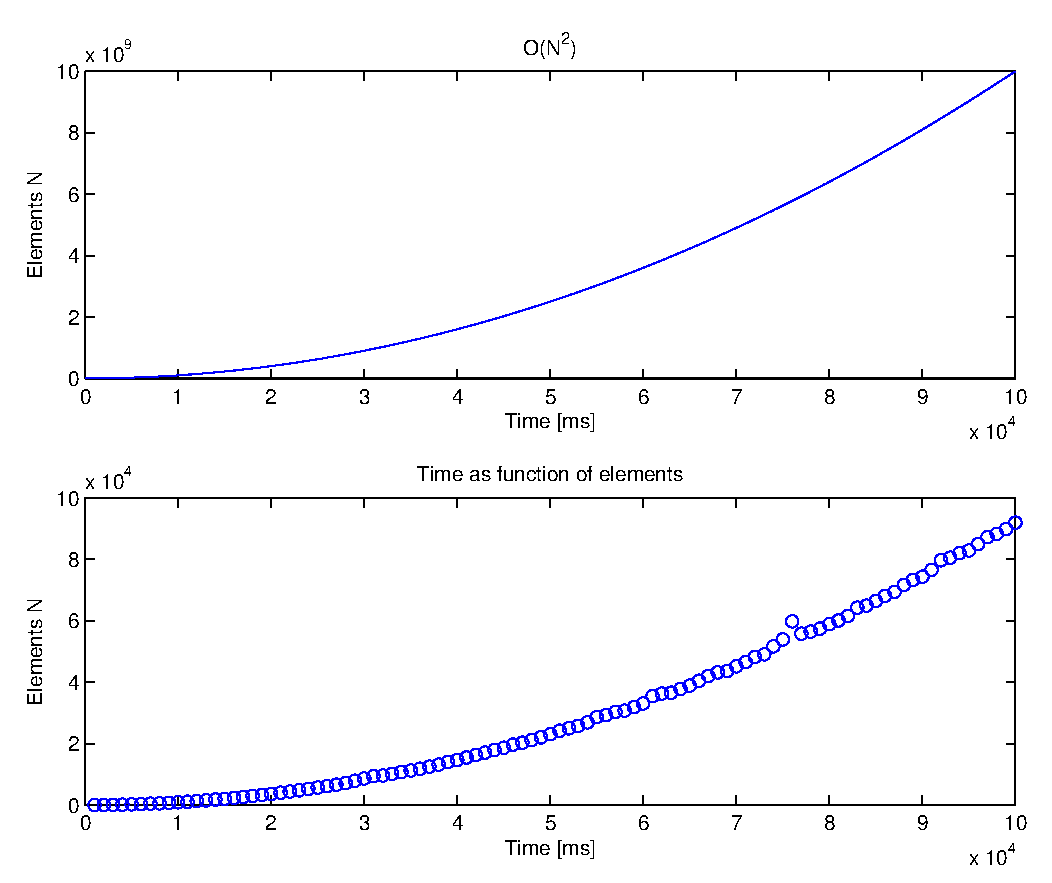
\includegraphics[width=1\textwidth]{./graphics/test1.eps}
\caption[tekst i indholdsfortegnelsen]{figurtekst}
\label{fig:}
\end{figure}
\newpage


\subsection{O(N Log(N)}
Figure \ref{fig:test2}


\todo[inline]{Description of the plot}
\begin{figure}[th!]
\centering
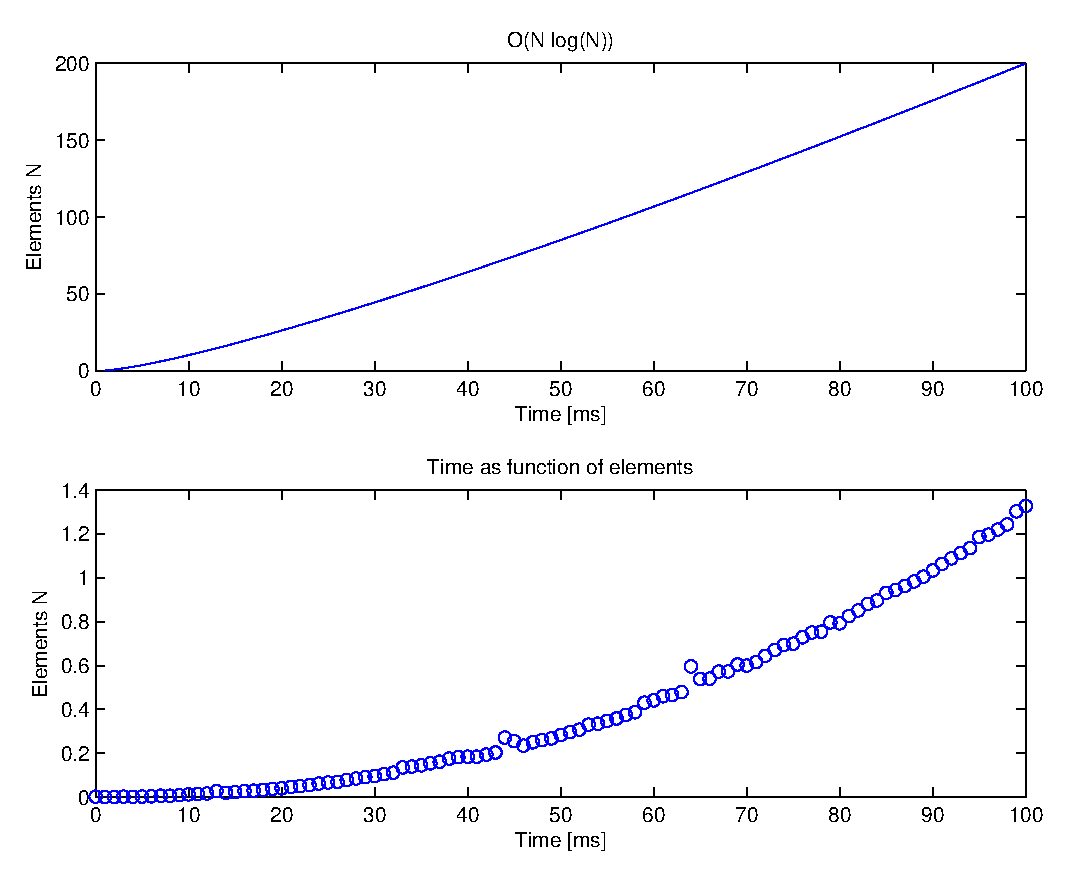
\includegraphics[width=1\textwidth]{./graphics/test2.eps}
\caption{Show plots of an ideal O(N log(N)) and data output from the algorithm.}
\label{fig:test2}
\end{figure}
